\documentclass{article}
\usepackage{graphicx} % Required for inserting images
\usepackage[linesnumbered,ruled,vlined]{algorithm2e}
\usepackage{algpseudocode}

\title{The Girvan-Newman Algorithm}
\author{Aaron Frye and Ben Lenox}
\date{November 2024}

\begin{document}

% \includegraphics[scale=0.1]{diagram.jpg}

\maketitle

\section{Overview of Algorithm}

The purpose of the Girvan-Newman Algorithm is to find communities---or areas of graphs with relatively high density.  Communities are groups of nodes that are relatively connected---the most connected community would be a clique.  This community detection is achieved by continuously removing edges based on a metric called edge betweenness centrality until the modularity of the graph reaches a certain point.  Edge betweenness centrality is a measure of how many shortest paths go over any given edge.  An edge that has more shortest paths going through it will have a higher edge betweenness centrality.  Modularity is a measurement of how well a given set of communities (set of sets of nodes) divides the graph into communities.  If the given communities have a high degree of connectivity intra-the communities, and are sparsely connected between the communities, modularity will be close to 1 (the maximum modularity value).  To enable the calculation of modularity, the algorithm must keep track of the connected components of the current graph (after edge removals). \\

The algorithm goes as follows: the edge betweenness centrality is calculated for every edge.  Then, the edge with the highest edge betweenness centrality is removed. The previous two steps are repeated until the modularity of the graph is higher than a given parameter for modularity.

\section{Pseudocode}

\begin{algorithm}[H]
\caption{$GirvanNewman(G, modBound)$}
\KwIn{Graph $G$ -- an undirected graph, Float $modBound$ -- a bound for the modularity so the algorithm knows when it is complete}
\KwOut{An undirected graph composed of all vertices and some edges of G, likely with more connected components representing communities}

$G2 \gets copy(G)$\;
$connectedComponents \gets DetectConnectedComponents(G, G.nodes)$\;
\While{$Modularity(G, connectedComponents) < modBound$}{
    $betweennessCentrality \gets CalculateEdgeBetweennessCentrality(G2)$\;
    $maxEdge \gets $ edge with max betweenness centrality in $G2$\;
    Remove $maxEdge$ from $G2$\;
    \ForEach{$nodeSet \in connectedComponents$}{
    	\If{$maxEdge.node1 \in nodeSet$}{
		$currComponent \gets nodeSet$\;
		break\;
	}
    }
    $newComponents \gets DetectConnectedComponents(G, currComponent)$\;
    \If{$newComponents.length == 2$}{
    Remove $currComponent$ from $connectedComponents$\;
    Add $newComponents$ to $connectedComponents$\;
    }
}

\Return{$G2$}\;
\end{algorithm}

\begin{algorithm}[H]
\caption{$DetectConnectedComponents(G, allNodes)$}
\KwIn{Graph $G$ -- an undirected graph, Node Set $allNodes$ -- a set of nodes of G to split into sets of nodes representing connected components}
\KwOut{A list of sets of nodes in G, each set representing one connected component}

$components \gets $ empty list\;
\While{$allNodes$ is not empty}{
	$visited \gets $ empty set\;
	$stack \gets $ arbitrary element removed from $allNodes$ inserted into an empty stack\;
	\While{$stack$ is not empty}{
		$currNode \gets stack.pop()$\;
		add $currNode$ to $visited$\;
		Remove $currNode$ from $allNodes$\;
		\ForEach{Node $n$ adjacent to $currNode$ in $G$}{
			\If{$n$ is not in $stack$ and $n$ is not in $visited$}{
				$stack.push(n)$\;
			}
		}
	}
	append $visited$ to $components$\;
}
\Return{$components$}\;
\end{algorithm}

\begin{algorithm}[H]
\caption{$Modularity(G, components)$}
\KwIn{Graph $G$ -- an undirected graph, List of Sets $components$ -- a list of sets of nodes representing the communities to use for G in the modularity calculation}
\KwOut{Integer -- the modularity of G}

$sum \gets 0$\;
$m \gets $ number of edges in $G$\;
\ForEach{Node $n1$ in $G.nodes$}{
	\ForEach{Node $n2$ in $G.nodes$}{
		\If{$n1$ is in the same component as $n2$}{
			$A \gets $ 1 if $G$ has edge ($n1$, $n2$)\;
			$d1 \gets $ degree of $n1$\;
			$d2 \gets $ degree of $n2$\;
			$sum \gets sum + A - ((d1 * d2) / (2 * m))$\;
		}
	}
}
\Return{$sum / (2 * m)$}\;
\end{algorithm}

\begin{algorithm}[H]
\caption{CalculateEdgeBetweennessCentrality(G)}
\KwIn{Graph $G$ -- an undirected graph}
\KwOut{Dictionary containing the the edges and their related betweenness centrality value}

$EBC \gets $ empty dictionary\;
\ForEach{Edge $e$ in $G.edges$}{
	$EBC[e] \gets 0$\;
}
\ForEach{Node $n$ in $G.nodes$}{
	$distanceDict \gets $ new Dictionary\;
	$distanceDict[n] \gets 0$\;
	$queue \gets $ new Queue\;
	$queue.enqueue(n)$\;
	$visited \gets $ empty set\;
	\While{$queue$ is not empty}{
		$currNode \gets queue.dequeue()$\;
		add $currNode$ to $visited$\;
		\ForEach{Node $u$ adjacent to $currNode$ in $G$}{
			\If{$u$ not in $visited$ and $u$ not in $queue$}{
				$distanceDict[u] \gets distanceDict[currNode] + 1$\;
				$queue.enqueue(u)$\;
			}
		}
	}
	$numShortestPaths \gets $ new Dictionary\;
	\ForEach{Node $u$ in $G.nodes$}{
		$numShortestPaths[u] \gets 0$\;
	}
	$numShortestPaths[n] \gets 1$\;
	$visited \gets $ empty set\;
	$distances \gets $ sort list of (key, value) pairs in $distanceDict$ by value\;
	\ForEach{($key$, $d$) in $distances$}{
		\ForEach{Node $pred$ adjacent to $key$ in $G$}{
			\If{distanceDict[pred] == $d$ - 1}{
				$numShortestPaths[key] \gets numShortestPaths[key] + numShortestPaths[pred]$\;
			}
		}
	}
	$edgeWeights \gets $new Dictionary\;
	\ForEach{Edge $e$ in $G$}{
		$edgeWeights[e] \gets 0$\;
	}
	\ForEach{($key$, $d$) in $distances$}{
		$sumIncoming \gets 0$\;
		\ForEach{Node $succ$ adjacent to $key$ in $G$}{
			\If{$distanceDict[succ] == d + 1$}{
				$sumIncoming \gets sumIncoming + edgeWeights[(key, succ)]$\;
			}
		}
		\ForEach{Node $pred$ adjacent to $key$ in $G$}{
			\If{$distanceDict[pred] == d - 1$}{
				$edgeWeights[(n, pred)] \gets (1 + sumIncoming) * (numShortestPaths[pred] / numShortestPaths[key])$\;
			}
		}
	}
	\ForEach{Edge $e$ in $edgeWeights$}{
		$EBC[e] \gets EBC[e] + edgeWeights[e]$\;
	}
}
\ForEach{Edge $e$ in $G.edges$}{
	$EBC[e] \gets EBC[e] / 2$\;
}
\Return{EBC}\;
\end{algorithm}

\section{Justification for Selection of Data Structures}

Each element of the implementation of the Girvan-Newman algorithm uses NetworkX's graphs.  This is because this algorithm acts on graphs to find communities.  NetworkX's graphs also have many useful built-in features like the ability to retrieve the graph as an adjacency list, the ability to check if an edge is in the graph, the ability to retrieve a set of all graph edges and nodes, and much more. \\

The Girvan-Newman function itself does not use any data structures unique to this function, but the component functions (algorithms) that are used to build the Girvan-Newman algorithm do.  We will be going over the selection of data structures for these component algorithms. \\

The DetectConnectedComponents algorithm uses a stack, a set, and a list of sets of nodes.  The stack is chosen because detecting these connected components is done using a depth-first search of the graph.  The set is used to keep track of which nodes have been visited in each depth-first search.  A set is useful because membership can be checked in constant time, which is required when completing a depth-first search.  A list of sets is used to keep track of connected components.  After every depth-first search, all nodes visited in that depth-first search are added to the list of sets as a set representing a connected component.  A set of sets cannot be used because sets are not hashable, so they cannot be elements of a set in python.  A list of sets is used for the aforementioned ability to check membership in constant time for any given set. \\

The algorithm to calculate modularity makes use of the list of sets created by the previous function.  This list of sets is used for its ability to provide constant-time set membership evaluation for each set in the list. \\

The algorithm used to calculate edge betweenness centrality uses a variety of data structures for a variety of purposes.  First, a dictionary is used to keep track of the edge betweenness centrality for each edge.  A dictionary is used to provide constant-time lookups for the betweenness centrality of any given edge.  The distance from a given node to all nodes in the graph is then calculated using a breadth-first search.  A queue is used for the breadth-first search.  A dictionary is used to store these distances---also to provide-constant time lookup of distances to the start node.  Another dictionary is created to store the number of shortest paths from the start node to each node in the graph---also to provide constant lookup time.  The distances dictionary previously mentioned is then turned into a list of (key, value) pairs in order to enable sorting (by value), which is necessary to calculate the number of shortest paths.  Yet another dictionary is then created to store edge weights (partial calculation of edge betweenness centrality for one start node).  This is also to provide constant lookup time, which is used when adding this value to the total edge betweenness centrality value stored in the initial dictionary.  The graph is then retrieved as an adjacency list to enable the calculation of edge weights.  The adjacency list is necessary so nodes adjacent to any given node can all be viewed in sequence for this calculation.

\section{Intuition for Correctness}

This algorithm computes communities in a graph by removing edges.  The remaining connected components are the computed communities.  The edges are removed via a metric called edge betweenness centrality.  The edge with the max betweenness centrality value is removed from the graph in each iteration.  The question then becomes: why is it that an edge with a high betweenness centrality value is likely to be an edge between two communities. \\

Edge betweenness centrality is a measure of how many shortest paths will pass over the given edge.  That is, if every shortest path between two nodes were computed, the edges that are used the most in these shortest paths will have the highest edge betweenness centrality. \\

Now, picture any graph, as below, with two very clear communities.  There is only one edge between these two communities (that edge being ("E", "D")).  Because of that fact, any shortest path between nodes in one community and nodes in the other community will have to pass through that edge.  We would therefore expect ("E", "D") to have a high edge betweenness centrality value. \\

\begin{center}
    \makebox[\textwidth]{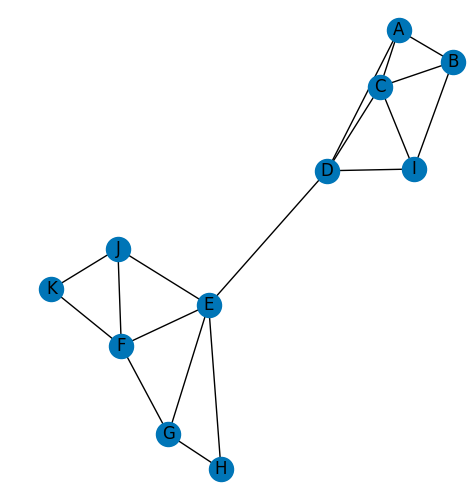
\includegraphics[scale=0.45]{test20.png}}
\end{center}

If we calculate the edge betweenness centrality values for this graph, we will see that ("E", "D") does, in fact, have the highest edge betweenness centrality value, by a significant margin.

\begin{center}
    \makebox[\textwidth]{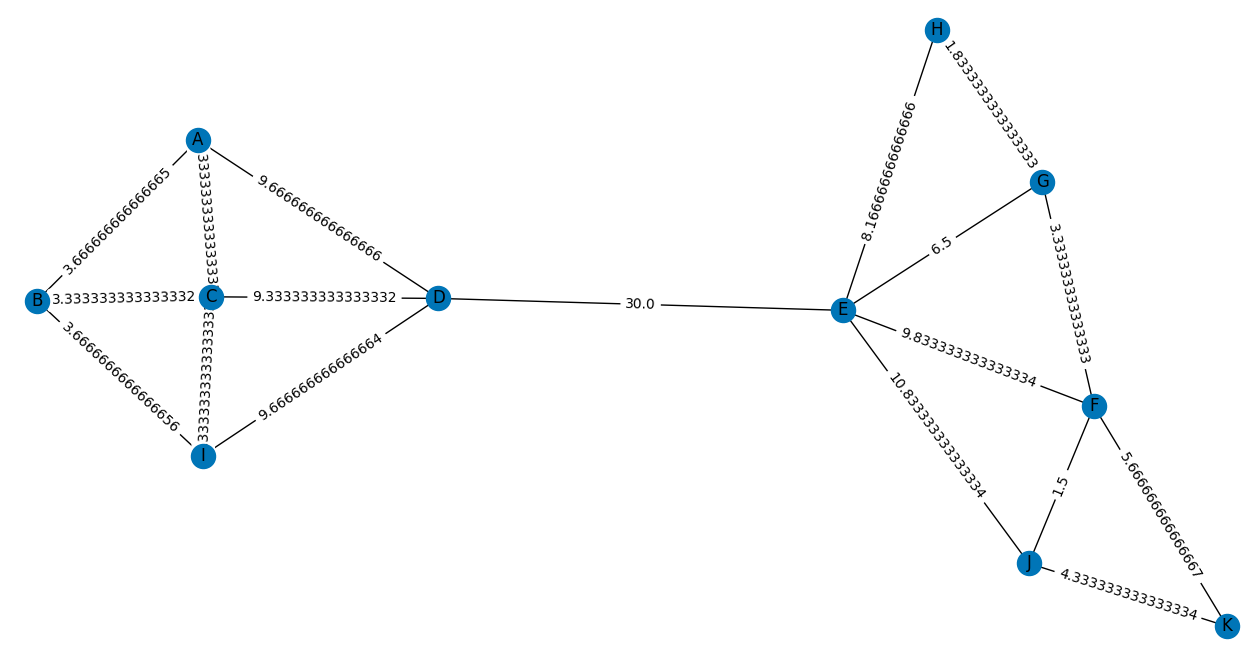
\includegraphics[scale=0.45]{test1.png}}
\end{center}

This would remain the case if there were exactly two edges between these two communities, but the difference would be more marginal, as some of the shortest paths between communities would go over one of these edges, and some would go over the other.  If we continued to add edges between the communities, the edge betweenness centrality values of these edges would continue to decrease until they were similar to the other edges within these communities.  At this point, it would make sense to say that the entire graph is one larger community rather than two smaller communities.

\section{Time Complexity Analysis}

Before the Girvan-Newman algorithm begins its main loop, connected components of the given graph are detected using the DetectConnectedComponents algorithm.  This is done in $\Theta(n + m)$ time using a breadth-first search.  In this algorithm, each node and each edge is iterated over exactly one time. \\

The Girvan-Newman algorithm has one main loop, which can run as many as m times.  This is because one edge is being removed in each iteration---the algorithm will stop if there are no edges (both in implementation, more explicitly, and because the modularity of the graph will be at its maximum value if there are no edges).  In each iteration, several things happen in non-constant time.  The modularity of the graph is calculated, the edge betweenness centrality of the graph is calculated (by far the most time-complex operation), the max edge is found, and the connected components list is updated. \\

The modularity calculation happens in $\Theta(n^2)$ time.  Constant time calculations are computed for each possible pair of nodes in the graph. \\

Edge betweenness centrality for the graph is calculated in $\Theta(n*(n + m))$ time.  This is because the main loop for the edge betweenness centrality calculation iterates over each of the nodes in the graph.  In each iteration, 3 breadth-first searches are performed.  The first finds the distance between the start node and each other node in the graph.  The second finds the number of shortest paths between the start node and each other node in the graph.  The third calculates edge weights for the edge betweenness centrality calculation for the starting node (a partial computation of edge betweenness centrality). \\

The max edge (with regard to betweenness centrality) is found in $\Theta(m)$ time.  The set of edges is searched for the max betweenness centrality by checking each edge once. \\

The connected components list is updated in $\Theta(n + m)$ time.  A breadth first search is done on the connected component that contained the removed edge using the DetectConnectedComponents algorithm.  If the one connected component turned into two, then the list of connected components is updated in $\Theta(n)$ time. \\

Putting this all together, the time complexity of the Girvan-Newman algorithm is $\Theta((n + m) + m*(n^2 + n*(n + m) + m + (n + m))) = \Theta((n + m) + m*(n*(n + m))) = \Theta(mn(n + m))$.  This makes the Girvan-Newman algorithm impractical for running on very large or very dense graphs, as it is very time-complex. \\


\section{Space Complexity Analysis}

The  Girvan-Newman algorithm has a relatively low space complexity compared to its extremely high time complexity.  This is because, while each component algorithm is run many times, the algorithm need only keep track of the latest computation of each algorithm.  Python's garbage collector can free up the previously used space. \\

Firstly, the Girvan-Newman algorithm must compute the connected components of the given graph.  This is done in $\Theta(n)$ space.  This algorithm keeps track of all visited nodes (as many as n nodes), all nodes on the stack (as many as n nodes), and a list of sets of nodes representing the connected components of the given graph (containing n nodes when the algorithm completes execution). \\

The Girvan-Newman algorithm must calculate the modularity of the graph once per iteration.  This does not require any additional space because the algorithm itself is already keeping track of the graph and the connected components---all that is required for the modularity calculation. \\

Edge Betweenness centrality is calculated n times as well.  Each calculation can be computed with a space complexity of $\Theta(m + n)$.  The edge betweenness centrality calculation initializes a dictionary with exactly m keys.  In each iteration of the main loop, the following data structures are created and used: a dictionary with n keys, a queue holding as many as n elements, a set containing n nodes, another dictionary containing n keys, a list containing n elements, and a dictionary containing m keys.  None of these data structures are retained between loops.  Edge betweenness centrality calculation therefore has a space complexity of $\Theta(n + m)$. \\

DetectConnectedComponents is also run n times, again having a space complexity of $\Theta(n)$. \\

Because none of these data structures are retained between iterations of the Girvan-Newman algorithm's main loop, the entire algorithm has a space complexity of $\Theta(n + m)$. \\

\section{Python Code}

\begin{verbatim}
import networkx as nx
import matplotlib.pyplot as plt
from collections import deque
from random import randrange

def sort_edge(tpl):
    return tuple(sorted(tpl))

def BFS(g, start):
    q = deque()
    q.append(start)
    result = {start: 0}
    visited = set()
    adj_list = dict(g.adjacency())
    while q:
        current = q.popleft()
        visited.add(current)
        for n in adj_list.get(current):
            if n not in visited and n not in q:
                result[n] = result[current] + 1
                q.append(n)
    return result

def num_shortest_path(g, dist_dict, start):
    result = dict((n, 0) for n in g.nodes())
    result[start] = 1
    visited = set()
    adj_list = dict(g.adjacency())
    dists = sorted(dist_dict.items(), key=lambda x: x[1])
    for n, d in dists:
        for pred in adj_list[n]:
            if dist_dict[pred] == d - 1:
                result[n] += max(1, result[pred])
    return result

def calculate_edge_weights(g, dist_dict, sp_dict):
    dists = sorted(dist_dict.items(), key=lambda x: x[1], reverse=True)
    edge_weights = {e : 0 for e in g.edges()}
    adj_list = dict(g.adjacency())
    for n, d in dists:
        sum_incoming = 0
        for succ in adj_list[n]:
            if dist_dict[succ] == d + 1:
                sum_incoming += edge_weights[sort_edge((n, succ))]
        for pred in adj_list[n]:
            if dist_dict[pred] == d - 1:
                edge_weights[sort_edge((n, pred))] = (1 + sum_incoming) * (sp_dict[pred] / sp_dict[n])
    return edge_weights

def calculate_edge_betweenness_centrality(g):
    for e in g.edges():
        g.edges[e]['betweenness'] = 0
    for n in g.nodes():
        dist_dict = BFS(g, n)
        sp_dict = num_shortest_path(g, dist_dict, n)
        edge_weights = calculate_edge_weights(g, dist_dict, sp_dict)
        for e in edge_weights:
            g.edges[e]['betweenness'] += edge_weights[e]
    for e in g.edges():
        g.edges[e]['betweenness'] /= 2

def path_exists(g, a, b):
    adj_list = dict(g.adj)
    stack = [a]
    visited = set()
    while stack:
        current = stack.pop()
        visited.add(current)
        if current == b:
            return True
        for n in adj_list[current]:
            if n not in stack and n not in visited:
                stack.append(n)
    return False

def same_component(components, n1, n2):
    n1_comp = set()
    for n_set in components:
        if n1 in n_set:
            n1_comp = n_set
            break
    return n2 in n1_comp

def modularity(g, components):
    sum_stuff = 0
    m = g.number_of_edges()
    for n1 in g.nodes:
        for n2 in g.nodes:
            if same_component(components, n1, n2):
                A = g.has_edge(n1, n2)
                d1 = g.degree(n1)
                d2 = g.degree(n2)
                sum_stuff += A - (d1*d2 / (2 * m))
    return sum_stuff / (2 * m)

def detect_connected_components(g, all_nodes = {}):
    components = []
    if not all_nodes: all_nodes = set(g.nodes)
    else: all_nodes = all_nodes.copy()
    adj_list = dict(g.adj)
    while all_nodes:
        visited = set()
        stack = [all_nodes.pop()]
        all_nodes.add(stack[0])
        while stack:
            current = stack.pop()
            visited.add(current)
            all_nodes.remove(current)
            for n in adj_list[current]:
                if n not in stack and n not in visited:
                    stack.append(n)
        components.append(visited)
    return components


def girvan_newman(g, mod_bound = 0.3):
    g2 = g.copy()
    connected_components = detect_connected_components(g2)
    while modularity(g, connected_components) < mod_bound and not nx.is_empty(g2):
        calculate_edge_betweenness_centrality(g2)
        try:
            max_edge = max(g2.edges(data=True), key=lambda e: e[2]['betweenness'])
        except:
            # print(e2.edges(data=True))
            break
        n1, n2 = max_edge[0:2]
        g2.remove_edge(n1, n2)
        curr_component = set()
        for node_set in connected_components:
            if n1 in node_set:
                curr_component = node_set
                break
        new_components = detect_connected_components(g2, curr_component)
        if len(new_components) == 2:
            connected_components.remove(curr_component)
            connected_components.extend(new_components)
    print(connected_components)
    return g2

def test(G, mb=0.3, show_ebc=False):
    G1 = G
    G2 = girvan_newman(G1, mb)

    if show_ebc:
        calculate_edge_betweenness_centrality(G1)
        edge_labels = round_dict(nx.get_edge_attributes(G1,'betweenness'))
        nx.set_edge_attributes(G1, edge_labels, "betweenness")

    fig, axes = plt.subplots(1, 2)
    pos = nx.spring_layout(G1)
    pos2 = nx.spring_layout(G2, k=0.75)

    nx.draw(G1, pos, ax=axes[0], with_labels=True)
    nx.draw(G2, pos, ax=axes[1], with_labels=True)
    # nx.draw(G1, pos, with_labels=True)

    if show_ebc:
        nx.draw_networkx_edge_labels(G1, pos, ax=axes[0], edge_labels = edge_labels)

    plt.show()

def random_community_structure(num_communities, community_sizes, intra_community_connections=0.65, inter_community_connections=0.05, mod_bound=0.4):
    if type(community_sizes) is tuple:
        arg1 = [randrange(community_sizes[0], community_sizes[1]) for _ in range(num_communities)]
    else:
        arg1 = [community_sizes] * num_communities

    arg2 = [[intra_community_connections if i == j else inter_community_connections for i in range(num_communities)] for j in range(num_communities)]

    return nx.generators.community.stochastic_block_model(arg1, arg2)

# Test 1
# G1 = random_community_structure(5, (4, 10))
# Test 2
# G1 = random_community_structure(7, (3, 8), intra_community_connections=0.8)
# Test 3
# G1 = random_community_structure(10, 10, intra_community_connections=0.8, inter_community_connections=0.02)
# Test 4
# G1 = random_community_structure(3, 50, inter_community_connections=0.02)
# Test 5
# G1 = random_community_structure(5, (5, 15))
# test(G1, 0.5)

# Test 6
# G1 = nx.fast_gnp_random_graph(100, 0.02)
# isolated_nodes = list(nx.isolates(G1))
# G1.remove_nodes_from(isolated_nodes)
# Test 7
# G1 = nx.fast_gnp_random_graph(40, 0.1)
# isolated_nodes = list(nx.isolates(G1))
# G1.remove_nodes_from(isolated_nodes)
# Test 8
G1 = nx.fast_gnp_random_graph(20, 0.1)
isolated_nodes = list(nx.isolates(G1))
G1.remove_nodes_from(isolated_nodes)
test(G1, 0.4)

\end{verbatim}

\section{Tests}

The general use case of this algorithm is to detect communities in graphs, so the main graphs that we will be using for the tests have some kind of community structure.  These graphs are randomly generated using networkX's community.stochastic\_block\_model graph generator, which allows you to specify a list of community sizes as well as the probability of an edge connection within each individual community, and the probability of an edge connection from each community to each other community.  A successful test would mean the detection of n distinct communities where n is the number of communities specified in the graph generation.  The communities that the algorithm detects should be clearly visible in the graph as it is before the Girvan-Newman algorithm is run on it.  The modularity bound is adjusted as necessary to achieve the most accurate output.  Listed below each test will be the communities detected by the algorithm, in the form of a list of sets of nodes.


\subsection{Test 1}
    \begin{center}
        \makebox[\textwidth]{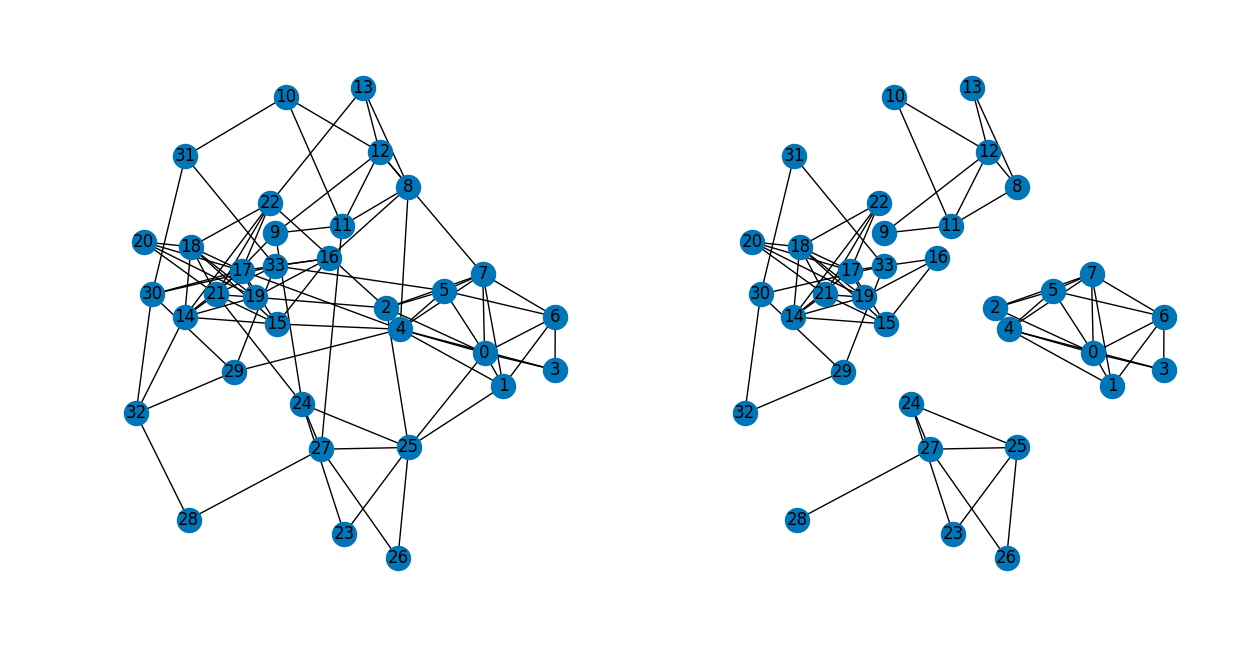
\includegraphics[scale=0.45]{test3.png}}
    \end{center}
    $[\{23, 24, 25, 26, 27, 28\}, \{8, 9, 10, 11, 12, 13\}, \{0, 1, 2, 3, 4, 5, 6, 7\}, \{32, 33, 29, 30, 31\}, \{14, 15, 16, 17, 18, 19, 20, 21, 22\}]$
\subsection{Test 2}
    \begin{center}
        \makebox[\textwidth]{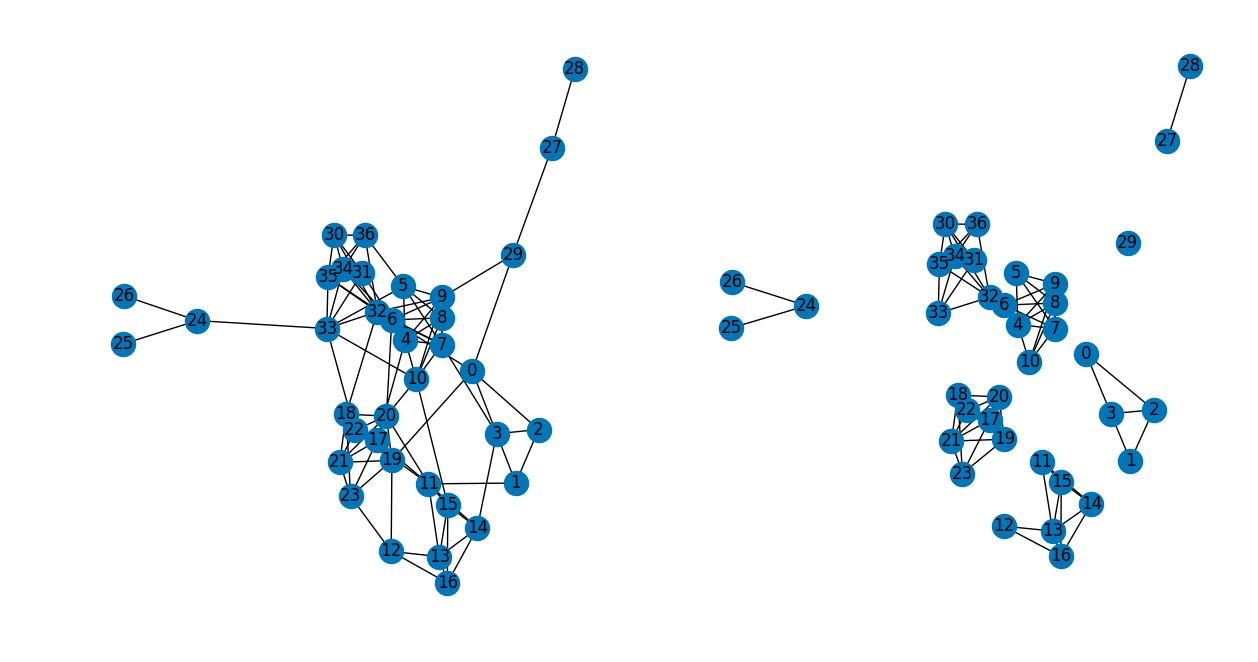
\includegraphics[scale=0.45]{test4.png}}
    \end{center}
    [\{24, 25, 26\}, \{27, 28\}, \{0, 1, 2, 3\}, \{29\}, \{11, 12, 13, 14, 15, 16\}, \{17, 18, 19, 20, 21, 22, 23\}, \{32, 33, 34, 35, 36, 30, 31\}, \{4, 5, 6, 7, 8, 9, 10\}]
\subsection{Test 3}
    \begin{center}
        \makebox[\textwidth]{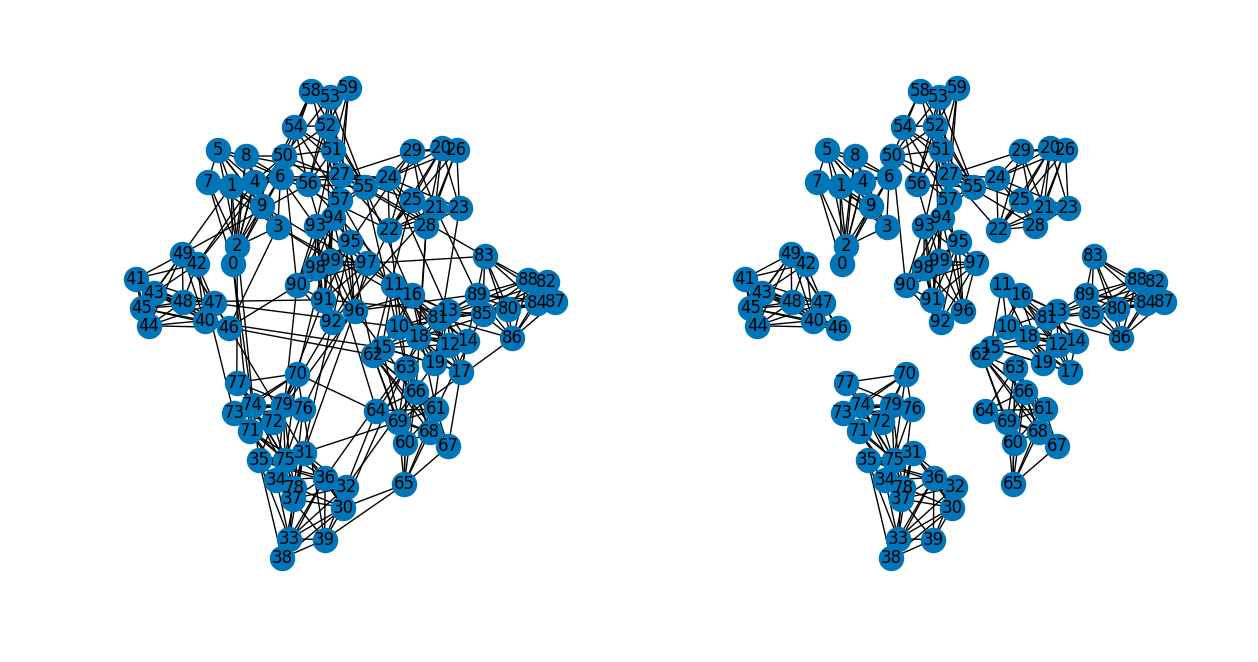
\includegraphics[scale=0.45]{test5.png}}
    \end{center}
    [\{40, 41, 42, 43, 44, 45, 46, 47, 48, 49\}, \{70, 71, 72, 73, 74, 75, 76, 77, 78, 79\}, \{80, 81, 82, 83, 84, 85, 86, 87, 88, 89\}, \{32, 33, 34, 35, 36, 37, 38, 39, 30, 31\}, \{50, 51, 52, 53, 54, 55, 56, 57, 58, 59, 90, 91, 92, 93, 94, 95, 96, 97, 98, 99\}, \{64, 65, 66, 67, 68, 69, 60, 61, 62, 63\}, \{10, 11, 12, 13, 14, 15, 16, 17, 18, 19\}, \{0, 1, 2, 3, 4, 5, 6, 7, 8, 9\}, \{20, 21, 22, 23, 24, 25, 26, 27, 28, 29\}]
\subsection{Test 4}
    \begin{center}
        \makebox[\textwidth]{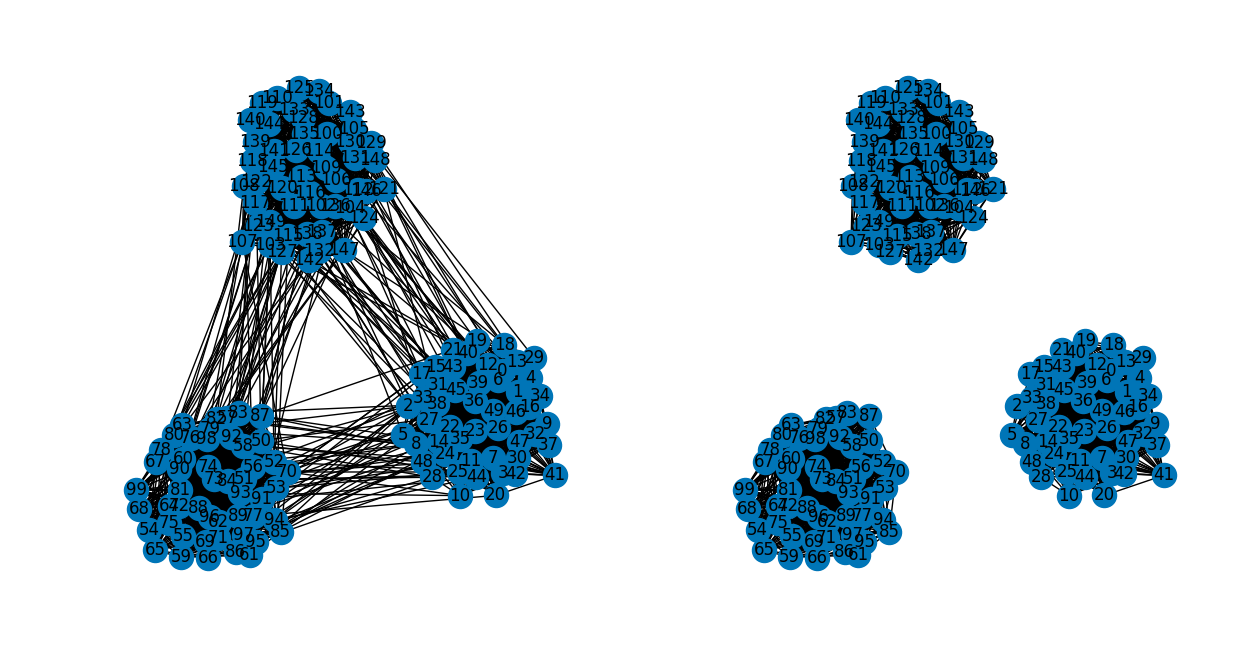
\includegraphics[scale=0.45]{test6.png}}
    \end{center}
      [\{128, 129, 130, 131, 132, 133, 134, 135, 136, 137, 138, 139, 140, 141, 142, 143, 144, 145, 146, 147, 148, 149, 100, 101, 102, 103, 104, 105, 106, 107, 108, 109, 110, 111, 112, 113, 114, 115, 116, 117, 118, 119, 120, 121, 122, 123, 124, 125, 126, 127\}, \{0, 1, 2, 3, 4, 5, 6, 7, 8, 9, 10, 11, 12, 13, 14, 15, 16, 17, 18, 19, 20, 21, 22, 23, 24, 25, 26, 27, 28, 29, 30, 31, 32, 33, 34, 35, 36, 37, 38, 39, 40, 41, 42, 43, 44, 45, 46, 47, 48, 49\}, \{50, 51, 52, 53, 54, 55, 56, 57, 58, 59, 60, 61, 62, 63, 64, 65, 66, 67, 68, 69, 70, 71, 72, 73, 74, 75, 76, 77, 78, 79, 80, 81, 82, 83, 84, 85, 86, 87, 88, 89, 90, 91, 92, 93, 94, 95, 96, 97, 98, 99\}]
\subsection{Test 5}
    \begin{center}
        \makebox[\textwidth]{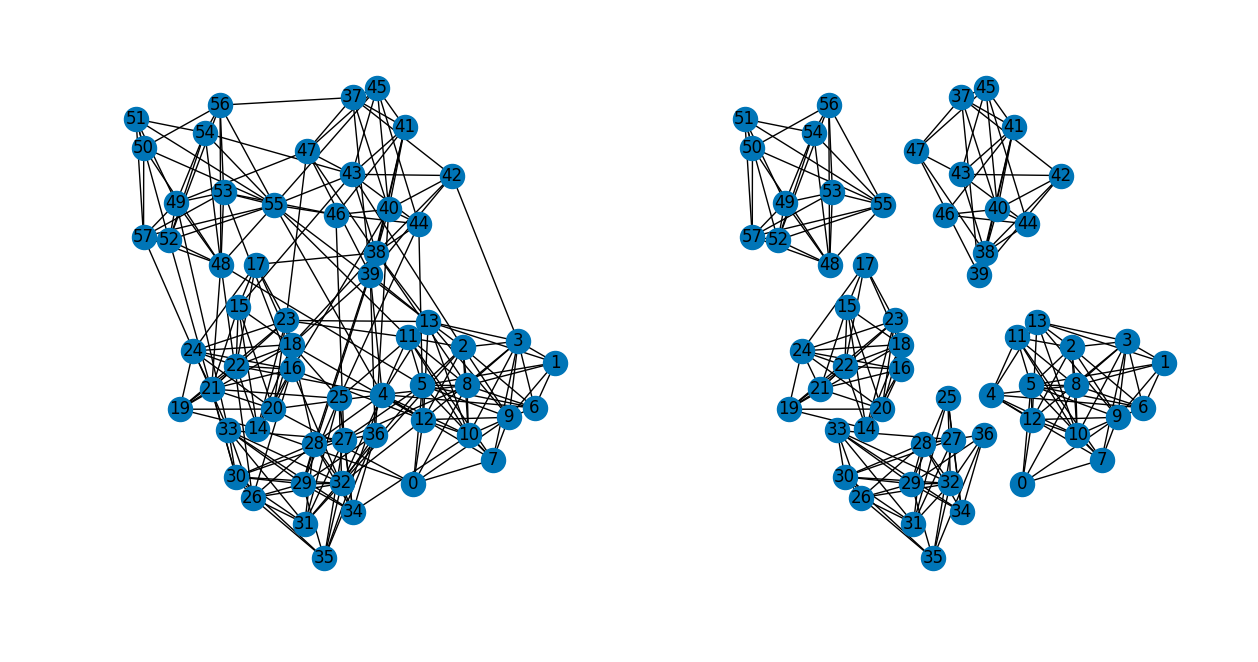
\includegraphics[scale=0.45]{test7.png}}
    \end{center}
    [\{48, 49, 50, 51, 52, 53, 54, 55, 56, 57\}, \{37, 38, 39, 40, 41, 42, 43, 44, 45, 46, 47\}, \{14, 15, 16, 17, 18, 19, 20, 21, 22, 23, 24\}, \{0, 1, 2, 3, 4, 5, 6, 7, 8, 9, 10, 11, 12, 13\}, \{32, 33, 34, 35, 36, 25, 26, 27, 28, 29, 30, 31\}]
\\ \\
As we can see, the algorithm seems to give an accurate result under varying conditions such as differences in community sizes and number of communities.  There is no great way to say that the algorithm we have implemented is completely correct, because the definition of "community" is mushy---being a relatively dense area of a graph.  The key word there is relatively.  Communities can be as dense or as sparse as makes sense in a given context. \\

Edge test cases would be graphs that do not have any inherent community structure.  The Girvan-Newman algorithm is built to find communities in situations where communities exist naturally, such as social networks.  The results of using the algorithm where no community structure exists naturally will be less useful than using it where communities do exist.  Below are some examples of edge cases.

\subsection{Test 6}
    \begin{center}
        \makebox[\textwidth]{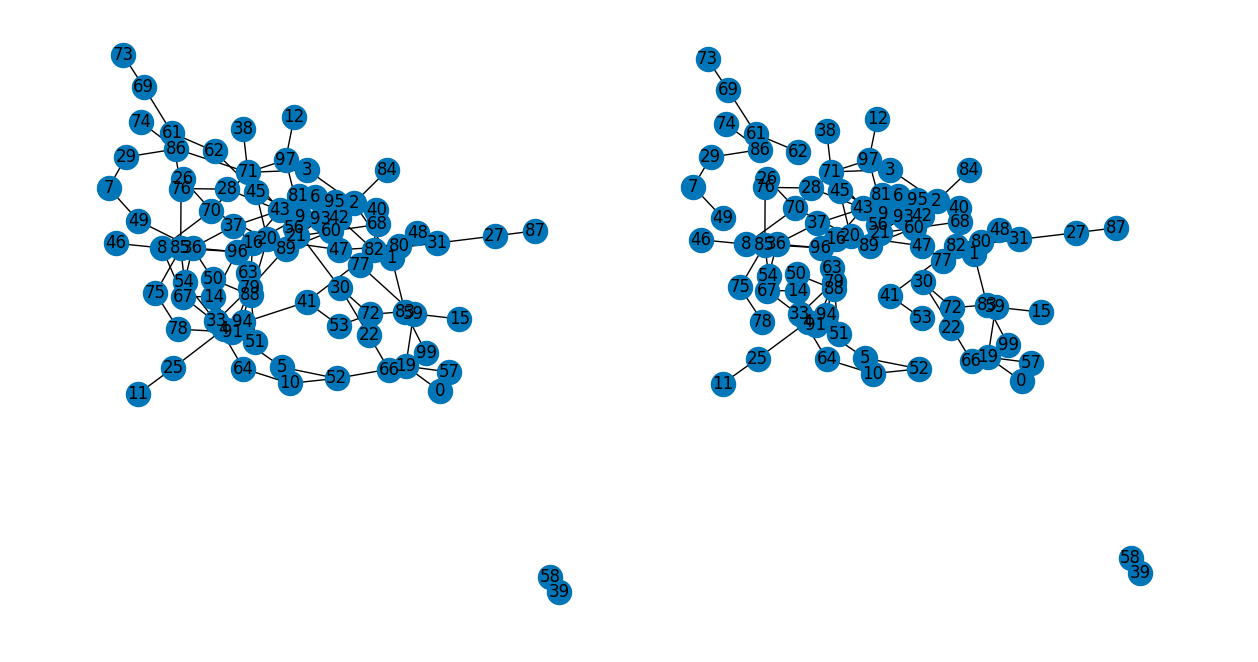
\includegraphics[scale=0.45]{test8.png}}
    \end{center}
    [\{48, 49, 50, 51, 52, 53, 54, 55, 56, 57\}, \{37, 38, 39, 40, 41, 42, 43, 44, 45, 46, 47\}, \{14, 15, 16, 17, 18, 19, 20, 21, 22, 23, 24\}, \{0, 1, 2, 3, 4, 5, 6, 7, 8, 9, 10, 11, 12, 13\}, \{32, 33, 34, 35, 36, 25, 26, 27, 28, 29, 30, 31\}]
\subsection{Test 7}
    \begin{center}
        \makebox[\textwidth]{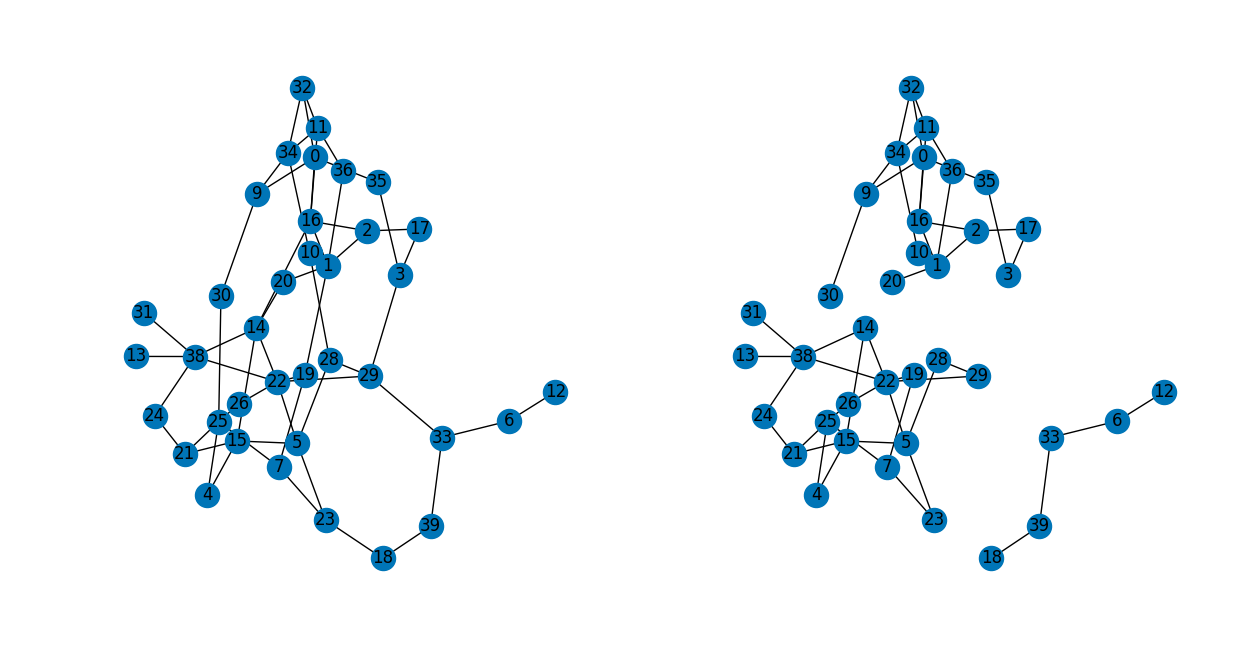
\includegraphics[scale=0.45]{test9.png}}
    \end{center}
    [\{33, 6, 39, 12, 18\}, \{0, 1, 2, 3, 35, 36, 34, 32, 9, 10, 11, 16, 17, 20, 30\}, \{4, 5, 38, 7, 13, 14, 15, 19, 21, 22, 23, 24, 25, 26, 28, 29, 31\}]
\subsection{Test 8}
    \begin{center}
        \makebox[\textwidth]{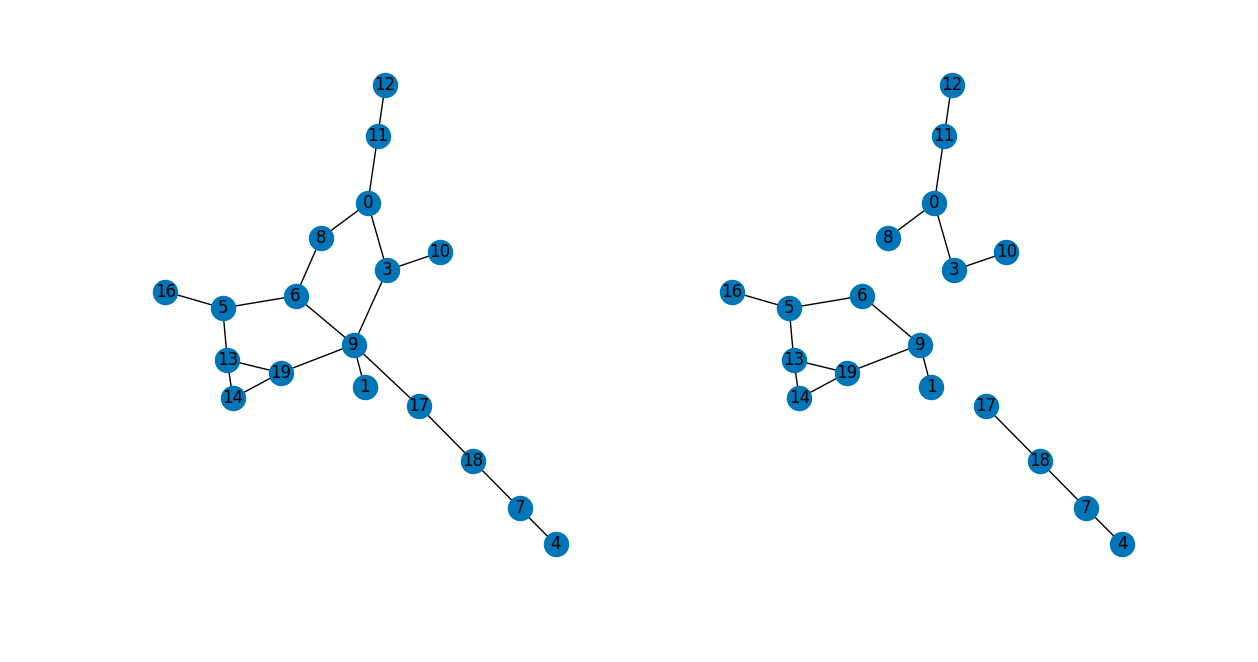
\includegraphics[scale=0.45]{test10.png}}
    \end{center}
    [\{12, 11, 0, 8, 3, 10\}, \{16, 5, 6, 9, 1, 19, 13, 14\}, \{17, 18, 7, 4\}]
\\ \\
As we can see, in these edge cases, the algorithm will still find groups of relatively densely connected nodes, but these node groups are much less clearly defined in the given graph.  The algorithm still appears to be working as intended.


\end{document}
